\documentclass{pj}
\usepackage{graphics}
\usepackage{amsmath}
\usepackage[mode=buildnew]{standalone}
\usepackage{tikz}
\renewcommand{\arraystretch}{1.5}

\begin{document}

\setcounter{page}{1}
\pjheader{Vol.\ x, y--z, 2014}

\title%
[Waveguide filter synthesis using mode-matching method]%
{Waveguide filter synthesis using mode-matching method}

\author{
  Dmitriy~A.~Dyomin\textsuperscript{*, 1},
  Nikolay~P.~Chubinsky\textsuperscript{1,2},
  Ivan~V.~Filatov\textsuperscript{1,3},
  Vasiliy~V.~Filatov\textsuperscript{4} and
  Nikolay~N.~Denisov\textsuperscript{5}
}

\footnote{\it Received date}
\setcounter{footnote}{0}
\footnote{\hskip-0.12in*\,
  Corresponding author: Dmitriy~Dyomin (demin.da@mipt.ru).}
\setcounter{footnote}{0}
\footnote{\hskip-0.12in\textsuperscript{1}
  Moscow Institute of Physics and Technology}
\setcounter{footnote}{0}
\footnote{\hskip-0.12in\textsuperscript{2}
  nchub940@yandex.ru}
\setcounter{footnote}{0}
\footnote{\hskip-0.12in\textsuperscript{3}
  ivfilatov@mail.ru}
\setcounter{footnote}{0}
\footnote{\hskip-0.12in\textsuperscript{4}
  Institute of Energy Problems for Chemical Physics (branch),
  vvfilatov1@gmail.com}
\setcounter{footnote}{0}
\footnote{\hskip-0.12in\textsuperscript{3} Institute of Problems of
  Chemical Physics of RAS, ndenisov@gmail.com}
\setcounter{footnote}{0}

\runningauthor{Dyomin et. al.}
\tocauthor{
  Dmitriy~A.~Dyomin,
  Nikolay~P.~Chubinsky,
  Ivan~V.~Filatov,
  Vasiliy~V.~Filatov and
  Nikolay~N.~Denisov
}

\begin{abstract}
  In this paper, a mode matching method is discussed in application to
  waveguide filter synthesis task. It is customized for analysis of
  particular waveguide filter with thick symmetric irises. Equivalent
  circuit model of thick iris discontinuities is also
  proposed. Parameters of the equivalent circuit are evaluated using
  mode-matching method. Using this model, an example filter for
  $Ka$-band has been designed. The performance of the filter has then
  been validated by the proposed mode-matching method and
  finite-elements method.
\end{abstract}

\section{Introduction}
\label{sec:introduction}

Filters are essential parts of modern high-frequency circuits.
Various filter types are used for different frequency bands, including
lumped-element networks for sub-GHz applications, while higher
frequencies require use of distributed elements such as microstrip or
waveguide resonators. Commonly, bandpass filters consist of resonators
coupled with each other. Several connections patterns are known,
including direct and indirect neighbours coupling. Indirect-coupled
filters may be realized as folded structures with couplings between
non-adjacent resonators or by using multi-mode resonators. They allow
more control over transfer function for the cost of increased
complexity and cost of fabrication. In this article, a narrowband
direct-coupled waveguide filter for $Ka$-band is considered. Coupling
is performed by irises symmetric around $yz$-plane
(Figure~\ref{fig:filter-drawing}).

\begin{figure}[h]
  \centering
  \includestandalone{images/model}
  \caption{Direct-coupled waveguide filter with symmetric irises}
  \label{fig:filter-drawing}
\end{figure}

There is a well-known theory of generic direct-coupled filters. A
complete set of equations for filter synthesis can be found in
\cite{cohn1957}. In this paper, a waveguide iris is represented by an
equivalent shunt inductance. It can be evaluated from geometric
parameters of the iris using relations from \cite{matthaei1980}.

However, this approximation works well only for the case of thin
irises. A practical $Ka$-band (wavelength
$\lambda \approx 8~\mathrm{mm}$) filter fabricated by milling contains
``thick'' irises ($h \approx 2~\mathrm{mm}$, so that $h/\lambda$ is not
negligible anymore). So, we aim at building equivalent circuit model
for this type of discontinuity. But at first let us consider direct
task of filter analysis.

\section{Waveguide filter analysis using mode-matching method}
\label{sec:mode-matching-method}

Conventional waveguide filter is a highly resonant structure with
large Q factor, so general purpose methods such as FEM, MoM or FDTD
converge slowly. Mode-matching method (MMM) has relaxed demands for
memory and computation time and is a preferred one for
waveguide-domain calculations. Of course, it is not so universal as
mesh methods as it requires determination of complete mode
set. This imposes no problem for the case of rectangular waveguide of
interest as its modes are known in analytical form.

A discussed waveguide filter is depicted on
Figure~\ref{fig:filter-drawing}. It consists of rectangular waveguide
sections connected with each other symmetrically around
$zy$-plane. Note that irises are also described as waveguide
sections. The only difference is the absence of propagating modes in
them. Filter is excited by a fundamental mode $TE_{01}$, so several
mode types are not excited throughout the structure:

\begin{itemize}
\item all $TM$ waves  
\item $TE_{n, m}, n \ne 0$ waves 
\item $TE_{0, 2m}$ waves (anti-symmetric around $yz$-plane while
  excitation $TE_{01}$ is symmetric).
\end{itemize}

Remaining are $TE_{0, 2m}$ waves only. Their
normalized $E_{y}$ components are represented by the following
relation:

\begin{equation}
  \label{eq:eigen_functions}
  E_y[TE_{0, 2m}] = F_{2m}^a(x) = \sqrt{\frac{2}{a}} \cos{\frac{2 \pi x m}{a}},
\end{equation}

where $a$ is the waveguide width. 

Overlapping matrix used to calculate reflection between adjacent
sections of widths $a$ and $b$ is for the case $a \le b$:
\begin{equation}
  \label{eq:overlapping}
  V_{mn} = \int\limits_{-a/2}^{a/2}F_m^a(x) F_n^b(x) dx =
  \begin{cases}
    \cfrac{4}{\pi} \cfrac{a^{-3/2} b^{-1/2} m
      (-1)^{\cfrac{m+1}{2}}}{\left(m/a\right)^2 -
      \left(n/b\right)^2} \cos{\left(\cfrac{\pi}{2}\cfrac{a}{b}n\right)}& \text{ if }\cfrac{m}{a} \ne \pm \cfrac{n}{b} \\
    \sqrt{\cfrac{a}{b}}~\text{ otherwise}
  \end{cases}
\end{equation}

Let $\mathbf{Q} = V_{mn}$,
$\mathbf{P} = \gamma_n^a/\gamma_m^b V_{nm}$, where $\gamma_n^a$ are
the propagation coefficients for mode $TE_{0, 2n+1}$ in a waveguide of
width $a$, then generalized $S$-parameters matrix of the waveguide
junction is (according to \cite{conciauro2000advanced}):

\begin{equation}
  \label{eq:s_matrix}
  \begin{array}{r@{}l}
    \mathbf{S}_{11} &{}= \left(\mathbf{I} + \mathbf{Q P}\right)^{-1} \left(\mathbf{I} + \mathbf{Q P}\right) \\
    \mathbf{S}_{12} &{}= 2\left(\mathbf{I} + \mathbf{Q P}\right)^{-1}\mathbf{Q} \\
    \mathbf{S}_{21} &{}= 2\left(\mathbf{I} + \mathbf{P Q}\right)^{-1}\mathbf{P} \\
    \mathbf{S}_{22} &{}= \left(\mathbf{I} + \mathbf{P Q}\right)^{-1}\left(\mathbf{I} - \mathbf{P Q}\right)
  \end{array}
\end{equation}

Here $\mathbf{I}$ are identity matrices of matching dimensions.

\begin{figure}
  \includestandalone{images/s12}
  \caption{Transmission coefficient matrix $S_{12}$ for a waveguide
    junction. Waveguide widths are $a=1$, $b=\sqrt{2}$ (in arbitrary
    units). Color represents the magnitude of $S_{12}$ matrix elements.}
  \label{fig:s12_matrix}
\end{figure}

An example solution for the case of connected waveguides of widths
$a = 1$ and $b = \sqrt{2}$ is shown on
Figure~\ref{fig:s12_matrix}. One can notice the quasi-diagonal
structure of the matrix, i.~e. energy is efficiently transferred
between modes numbers of which follow the simple equation $m/n =
a/b$. This results from a specific form of overlapping matrix in
Equation.~\ref{eq:overlapping}. Its values are close to $\sqrt{a/b}$
on quasi-diagonal indices and decrease rapidly on off-diagonal
elements. If $V_{mn}$ matrix axial ratio is unbalanced (i.~e. other than
$a/b$), then modes that do not have quasi-diagonal counterparts
undergo non-physical reflection. That's why increasing number of
accounted modes in one section only does not really improve
calculation precision. So, calculations described herein have been
carried out using matrices with balanced axial ratio.

Generalized $S$-matrix of a waveguide is as simple as
\begin{equation}
  \label{eq:waveguide_element}
  \mathbf{S}_{11} = \mathbf{S}_{22} = 0, \quad
  \mathbf{S}_{12} = \mathbf{S}_{21} = 
  \begin{bmatrix}
    e^{-\gamma_1} & 0 & \dots & 0 \\
    0 & e^{-\gamma_2} & \dots & 0 \\
    \vdots & \vdots & \ddots & \vdots \\
    0 & 0 & \dots & e^{-\gamma_N}
  \end{bmatrix}
\end{equation}

where $\gamma_n$ is still a propagation coefficient (real positive for
evanescent waves).

By knowing numeric values for generalized $S$-matrices for all the
elements of the waveguide filter, one can combine them to produce
generalized $S$-matrix of the whole filter. If
$\mathbf{A}, \mathbf{B}$ are the generalized $S$ matrices, then the
generalized $S$-matrix of the cascaded network
$\mathbf{A} \circ \mathbf{B}$ is

\begin{equation}
  \begin{array}{r@{}l}
    \mathbf{S}_{11} &{}=  \mathbf{A}_{11} + \mathbf{A}_{12} \left(\mathbf{I} - \mathbf{B}_{11}\mathbf{A}_{22}\right)^{-1} \mathbf{B}_{11} \mathbf{A}_{21} \\
    \mathbf{S}_{12} &{}=  \mathbf{A}_{12} \left(\mathbf{I} - \mathbf{B}_{11}\mathbf{A}_{22}\right)^{-1} \mathbf{B}_{12} \\
    \mathbf{S}_{21} &{}=  \mathbf{B}_{21} \left(\mathbf{I} - \mathbf{A}_{22}\mathbf{B}_{11}\right)^{-1}\mathbf{A}_{21} \\
    \mathbf{S}_{22} &{}=  \mathbf{B}_{22} + \mathbf{B}_{21}\left(\mathbf{I} - \mathbf{A}_{22}\mathbf{B}_{11}\right)^{-1}\mathbf{B}_{12} \\
  \end{array}
  \label{eq:cascaded_s}  
\end{equation}

Using equation~\eqref{eq:cascaded_s} is not the only way to find
cascaded network parameters. One could convert scattering parameters
$S$ to transmission parameters $T$ as described in
\cite{frei2008}. Cascading is much simpler in terms of
$T$-matrices. Resultant $T$-matrix is a matrix product of
$T$-matrices of the cascaded network elements. However, conversion
between $S$-matrix and $T$-matrix forms is not that straightforward:
\begin{equation}
  \label{eq:s_to_t}
  \begin{array}{r@{}l}
    \mathbf{T}_{11} &{}= \mathbf{S}_{12} - \mathbf{S}_{11}\mathbf{S}_{21}^{-1}\mathbf{S}_{22} \\
    \mathbf{T}_{12} &{}= \mathbf{S}_{11}\mathbf{S}_{21}^{-1} \\
    \mathbf{T}_{21} &{}= -\mathbf{S}_{21}^{-1}\mathbf{S}_{22} \\
    \mathbf{T}_{22} &{}= \mathbf{S}_{21}^{-1}
  \end{array}
\end{equation}

As pointed out in \cite{frei2008}, $\mathbf{S}_{21}$ block of
generalized $\mathbf{S}$-matrix is rectangular, so its inverse
$\mathbf{S}_{21}^{-1}$ is ambiguous and conversion between S- and
T-matrices results in loss of information. By contrast,
equation~\eqref{eq:cascaded_s} contains inverse values of square
matrices only.

Equations~\eqref{eq:overlapping} to \eqref{eq:cascaded_s} fully define
generalized $S$-matrix for the whole waveguide filter thus
accomplishing filter analysis task.

\section{Filter synthesis using equivalent circuit}
\label{sec:filter-synth}

Iris discontinuities in the discussed filter are modeled by shunt
inductances shown on Figure~\ref{fig:circuit:1}a. Shunt inductance can
be converted to impedance inverter using equations from
\cite{pozar2012microwave} thus yielding more general equivalent
circuit shown on Figure~\ref{fig:circuit:1}b. However, thin iris model
does not work well for $Ka$ band (wavelength $\lambda \approx 8~mm$)
with typical iris thickness $h \approx 2~mm$.

\begin{figure}[h]
  \begin{tabular}{cc}
    \includestandalone{images/schematic:inductors} & \includestandalone{images/schematic:thick_iris}
    \\
    a) & c) \\
    & \\
    \includestandalone{images/schematic:inverters} & \\
    b) & \\
  \end{tabular}
  
  \caption{Waveguide filter equivalent circuit.  a) $N$-section
    direct-coupled filter equivalent circuit, b) $N$-section filter
    equivalent circuit using impedance inverters, c) single thick
    iris equivalent circuit (also used as single inverter equivalent circuit).}
  \label{fig:circuit:1}
\end{figure}

Non-zero iris thickness results in additional phase shift which can be
modeled by attaching pieces of transmission lines to shunt inductance
(Figure~\ref{fig:circuit:1}c).  This is a symmetric $T$-network built
of a shunt inductor of impedance $X$ and two transmission lines
(electrical lengths $\theta/2$, wave impedance $Z_0$). Transmission
matrix is then
\begin{equation}
  \label{eq:abcd_matrix}
  \begin{array}{r@{}l}
  \begin{bmatrix}
    A & B \\
    C & D
  \end{bmatrix}
        = & 
  \begin{bmatrix}
    \cos{\theta/2} & j Z_0 \sin{\theta/2} \\
    j/Z_0 \sin{\theta/2} & \cos{\theta/2}
  \end{bmatrix}
  \begin{bmatrix}
    1 & 0 \\
    -j/X & 1
  \end{bmatrix}
  \begin{bmatrix}
    \cos{\theta/2} & j Z_0 \sin{\theta/2} \\
    j/Z_0 \sin{\theta/2} & \cos{\theta/2}
  \end{bmatrix} \\
    & \\
    = &
        \begin{bmatrix}
          \cfrac{Z_0}{2 X} \sin{\theta} + \cos{\theta} & j Z_0
          \left(\sin{\theta + \cfrac{Z_0}{2 X}
              \left(1-\cos{\theta}\right)}\right) \\
          \cfrac{j}{Z_0} \left(\sin{\theta} - \cfrac{Z_0}{2 X} (1 +
            \cos{\theta})\right) & \cfrac{Z_0}{2 X} \sin{\theta} + \cos{\theta}
        \end{bmatrix}
  \end{array}
\end{equation}
Converting ABCD-parameters to S-matrix, one determines:
\begin{equation}
  \label{eq:abcd_to_s}
  \begin{array}{r@{}l}
    S_{11} = S_{22} & = - \cfrac{e^{-j\theta}}{1 + 2jX/Z_0} \\
    S_{12} = S_{21} & = \cfrac{2j X}{Z_0} \cfrac{e^{-j\theta}}{1 + 2jX/Z_0} \\
  \end{array}
\end{equation}
So, equivalent circuit parameters may be calculated using S-parameters:
\begin{equation}
  \label{eq:equivalent_circuit}
  \cfrac{X}{Z_0} =
  \cfrac{1}{2}\sqrt{\cfrac{1}{\left|S_{11}\right|^2}-1} , \quad\quad
  \theta = -\arccos{\left|S_{11}\right|} - \arg{\left(-S_{11}\right)}
\end{equation}

S-parameters, in turn, depend on geometry of the particular iris and
are evaluated numerically using mode-matching method described in
the previous section. Results of these calculations are shown on
Figure~\ref{fig:equiv-circuit} for iris thickness $h = 2~mm$.

\begin{figure}[h]
  \begin{tabular}{cc}
    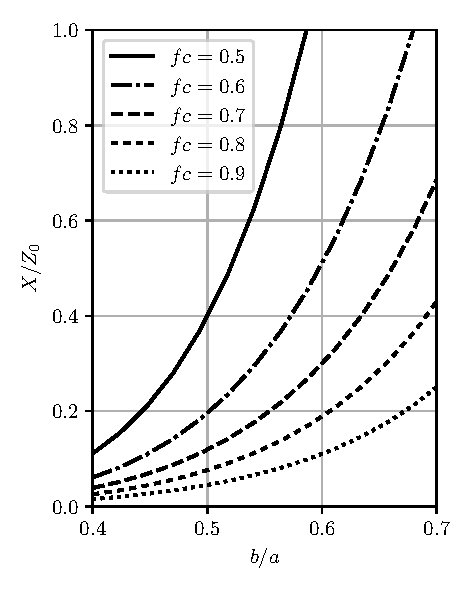
\includegraphics{images/impedance} &
                                           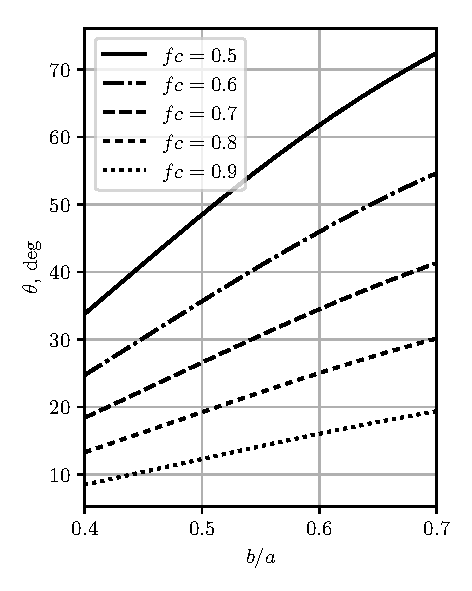
\includegraphics{images/theta}
    \\
    a) & b) \\
  \end{tabular}
  \caption{Equivalent circuit parameters for iris thickness $h = 2~mm$
    (waveguide width $a = 7.112~mm$). Parameter
    $fc = F_{cutoff}/F_{center}$ is the normalized cutoff
    frequency. a) equivalent impedance $X/Z_0$, b) equivalent
    transmission line length $\theta$
    (cf. Figure~\ref{fig:circuit:1}).}
  \label{fig:equiv-circuit}
\end{figure}


Impedance inverter's equivalent circuit is similar to that of thick
iris and depicted on Figure~\ref{fig:circuit:1}c. Conversion between
these representations is performed by equations from \cite{pozar2012microwave}:
\begin{equation}
  \label{eq:impedance_transformer}
  \cfrac{X_i}{Z_0} = \cfrac{K_i/Z_0}{(K_i/Z_0)^2-1},
  \quad
  \theta_i = - 2 \tan^{-1}{\left(\cfrac{K_i}{Z_0}\right)}
\end{equation}

Note that $\theta_i < 0$, i.~e. it is subtracted from adjacent half-wave
resonators.

Filter network shown on Figure~\ref{fig:circuit:1}b is similar to a
well-known problem of a capacitively-coupled microstrip filter. The
design procedure described in \cite{pozar2012microwave} is as follows:
\begin{itemize}
\item choose low-pass filter prototype (maximally flat, equal ripple, etc.)
\item determine selected filter's prototype values
  $g_0, g_1, \dots, g_{N+1}$ (cases for maximally-flat and
  equal-ripple filters are considered in \cite{matthaei1980})
\item determine transformation coefficients:
  \begin{equation}
    \begin{array}{r@{}l}
      \cfrac{K_1}{Z_0} &{}= \sqrt{\cfrac{2}{\pi} \cfrac{g_0g_1}{\Delta}}, \\
      \dots \\
      \cfrac{K_i}{Z_0} &{}= \cfrac{2}{\pi \Delta}\sqrt{g_i g_{i+1}} \\
      \dots \\
      \cfrac{K_N}{Z_0} &{}= \sqrt{\cfrac{2}{\pi} \cfrac{g_N g_{N+1}}{\Delta}}
    \end{array}
    \label{eq:trans_coeff}    
  \end{equation}
  where $\Delta = (F_{max}-F_{min})/F_{center}$ -- fractional
  bandwidth of the filter
\item determine line lengths $l^{\prime}_i = \Lambda_g/2$, where
  $\Lambda_g = \lambda / \sqrt{1-(F_{cutoff}/F_{center})^2}$ is the
  wavelength in waveguide at center frequency.
\end{itemize}

Given $K_i$ and $l^{\prime}_i$, one can determine $X_i/Z_0$ and
$l_i$ using equation~\eqref{eq:impedance_transformer}. A final step
is to use mode-matching model together with
equation~\eqref{eq:equivalent_circuit} and
Figure~\ref{fig:equiv-circuit} to evaluate irises' widths
$b_i$ and waveguide section lengths $L_i$.

The procedure described herein has been used to synthesize $Ka$-band
filter for a standard WR28 flange (width $a = 7.112~mm$) for the
following set of parameters:
\begin{itemize}
\item frequency band $F_{center} = 30.1~GHz \pm 5.1\%$
\item Tchebyshev filter, order $n = 6$, ripple 0.1~dB
\item cutoff frequency for fundamental mode of WR28 waveguide is $F_{cutoff} = 0.7 F_{center}$
\end{itemize}

\begin{table}

  \begin{tabular}{cc}
  \begin{tabular}{|l|l|l|}
    \hline
    $i$ & $X_i/Z_0$, mm & $l_i$, deg \\ \hline
    1 & 0.424 & 152.9 \\ \hline
    2 & 0.125 & 167.7 \\ \hline
    3 & 0.093 & 169.6 \\ \hline
    4 & 0.090 & 169.6 \\ \hline
    5 & 0.093 & 167.7 \\ \hline
    6 & 0.125 & 152.9 \\ \hline
    7 & 0.424 & \\ \hline
  \end{tabular} &
  \begin{tabular}{|l|l|l|}
    \hline
    $i$ & $b_i$, mm & $L_i$, mm \\ \hline
    1 & 4.56 & 4.68 \\ \hline
    2 & 3.59 & 5.50 \\ \hline
    3 & 3.39 & 5.63 \\ \hline
    4 & 3.36 & 5.63 \\ \hline
    5 & 3.39 & 5.50 \\ \hline
    6 & 3.59 & 4.68 \\ \hline
    7 & 4.56 & \\ \hline
  \end{tabular} \\
    a) & b) 
  \end{tabular}
  \caption{Proposed filter parameters: a) -- equivalent circuit
    parameters, b) -- filter dimensions.}
  \label{tab:filter_dimensions}
\end{table}

Equivalent circuit parameters for this filter are shown in
Table~\ref{tab:filter_dimensions}a. Using these data, filter
dimensions have been evaluated and are shown in
Table~\ref{tab:filter_dimensions}b. $S$-parameters of the designed
filter has been calculated using 3 different methods: equivalent
circuit model, mode matching method and FEM with the help of commercial
software (HFSS). Results are presented on
Figure~\ref{fig:transfer-function}.

\begin{figure}[h]
  \centering
  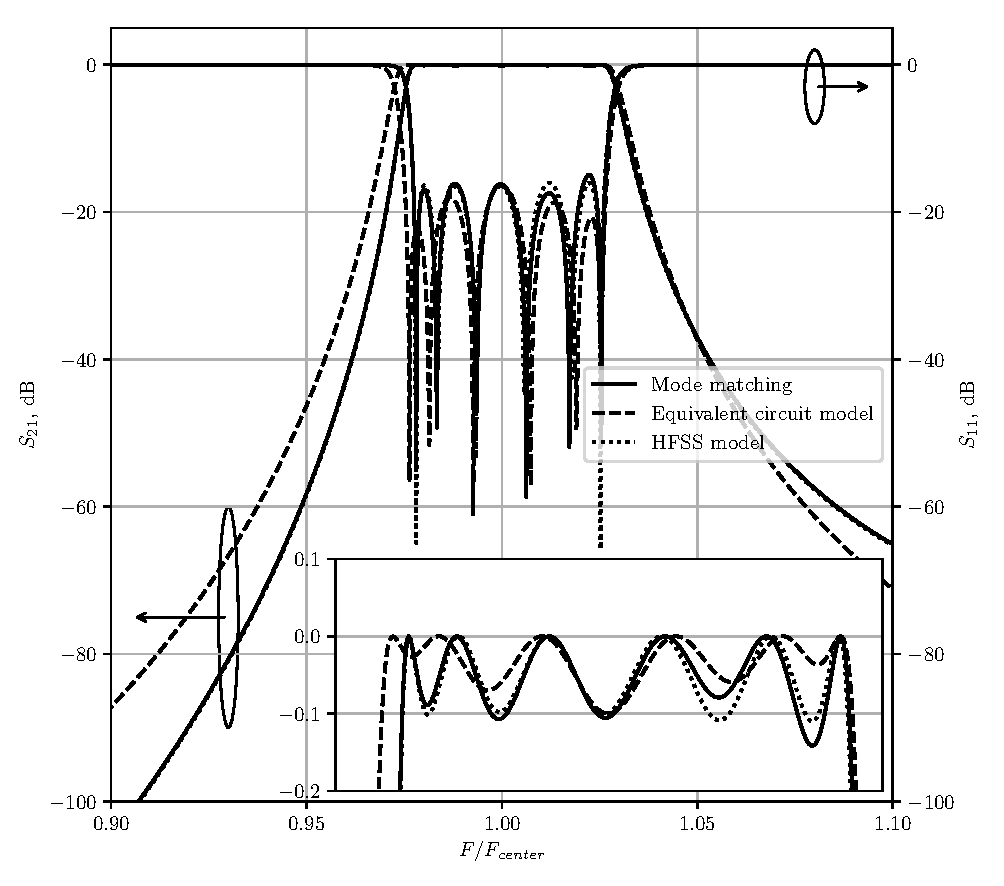
\includegraphics{images/reflections}
  \caption{Filter transfer function and reflection coefficient
    calculated using various methods: mode matching method (solid
    line), equivalent circuit method (dashed line) and finite elements
    method (dotted line).}
  \label{fig:transfer-function} 
\end{figure} 

FEM and MMM yield almost the same result with slight differences in
the pass-band that can be accounted for by finite precision of the
numerical methods. However, computation time for mode matching is
reduced drastically compared to the FEM: HFSS v15 calculations took 1
hour 36 minutes on desktop with Intel Core i7-2600, while the same
results have been obtained using Python (Numpy) code implementing MMM
in 49 seconds on the same hardware. Pass-band return loss is less than
$-15~dB$. As for equivalent circuit model, it is the fastest yet the
least accurate. Besides, this model shows systematic discrepancies in
selectivity: it is higher for $F < F_{center}$ and lower for
$F > F_{center}$ than calculated using MMM of FEM.

\section{Conclusion}
\label{sec:conclusion}
In this paper, an application of mode-matching method for waveguide
filter analysis and synthesis is discussed. This method has lower
demands on CPU time and memory compared to conventional mesh-based
techniques such as FEM.

The proposed thick iris model allowed applying conventional synthesis
procedure for direct-coupled waveguide filter with thick irises. A
band-pass filter has been designed using this procedure. Its center
frequency is $30.1~GHz$, bandwidth is $5\%$. The designed filter is
quite compact (overall length $L = 45.62~mm$, from
Table~\ref{tab:filter_dimensions}b) and can be used in high-speed
satellite transmission lines for separating up- and down-link signals
for duplex operation. Simulations using various computational methods
are consistent with each other.

HFSS models and developed Python scripts are available on
\texttt{https://github.com/dmitrodem/pier\_filter}.

\bibliography{db}{}
\bibliographystyle{pier}
\end{document}
%%% Local Variables:
%%% mode: latex
%%% TeX-master: t
%%% TeX-command-extra-options: "-shell-escape"
%%% End: